\documentclass{article}
\usepackage{amsmath}
\usepackage{graphicx}
\usepackage{hyperref}
\usepackage[utf8]{inputenc}
\usepackage[russian]{babel}

\begin{document}

\title{Нормализующие потоки и Римановы непрерывные нормализующие потоки}
\author{}
\date{}
\maketitle

\begin{abstract}
В данном эссе рассматриваются нормализующие потоки (NF) и их расширение в виде Римановых непрерывных нормализующих потоков (RCNF). NF представляют собой семейство моделей, которые преобразуют простую базовую плотность в сложную целевую плотность через обратимое и дифференцируемое преобразование. RCNF расширяют это понятие на римановы многообразия, позволяя более гибкое и точное моделирование распределений данных на криволинейных пространствах. В эссе приводятся формальные определения NF и RCNF, обсуждаются их математические основы и подчеркиваются их применения в различных областях.
\end{abstract}

\section{Введение}

Нормализующие потоки (NF) стали мощным инструментом в области машинного обучения и статистики для моделирования сложных вероятностных распределений. Путем преобразования простой базовой плотности, такой как гауссово распределение, в сложную целевую плотность через обратимое и дифференцируемое отображение, NF позволяют эффективно выполнять выборку и оценку плотности. Эта возможность нашла применение в различных областях, включая генеративное моделирование, вариационное выведение и оценку плотности.

Однако традиционные NF ограничены евклидовыми пространствами, что может быть неподходящим для данных, естественно расположенных на криволинейных многообразиях. Для решения этой проблемы были введены Римановы непрерывные нормализующие потоки (RCNF). RCNF расширяют концепцию NF на римановы многообразия, позволяя более гибкое и точное моделирование распределений данных на криволинейных пространствах. Включая геометрию многообразия через его метрический тензор, RCNF могут захватывать внутреннюю структуру данных, что приводит к улучшению производительности в задачах, таких как обучение на многообразиях и генерация данных на многообразиях.

В этом эссе мы предоставим всесторонний обзор NF и RCNF. Мы начнем с определения NF и обсуждения их математических основ. Затем мы введем понятие римановых многообразий и необходимые геометрические инструменты, такие как метрический тензор и аффинная связность. Наконец, мы формально определим RCNF и исследуем их применения и преимущества по сравнению с традиционными NF.

\section{Нормализующие потоки (NF)}

\subsection{Определение}

Нормализующие потоки (NF) представляют собой семейство моделей, которые преобразуют простую базовую плотность (например, гауссовскую) в сложную целевую плотность через обратимое и дифференцируемое преобразование.

Пусть \( p_Z(z) \) — базовая плотность, а \( f: \mathbb{R}^d \rightarrow \mathbb{R}^d \) — обратимое преобразование. Тогда плотность целевого распределения \( p_X(x) \) определяется как:

\begin{equation}
    p_X(x) = p_Z(f^{-1}(x)) \left| \det \left( \frac{\partial f^{-1}(x)}{\partial x} \right) \right|
    \label{eq:nf_density}
\end{equation}

Обучение NF сводится к нахождению оптимального преобразования \( f \), которое минимизирует расхождение между \( p_X(x) \) и целевой плотностью.

\section{Риманова геометрия}

\subsection{Определение}

Многообразие \( M \) — это топологическое пространство, локально похожее на евклидово пространство.

Метрический тензор \( g \) определяет локальную метрику на многообразии, т.е. способ измерения расстояний и углов.

Аффинная связность \( \nabla \) определяет параллельный перенос векторов на многообразии и, следовательно, кривизну.

\section{Римановы непрерывные нормализующие потоки (RCNF)}

\subsection{Идея}

RCNF расширяет классические NF, позволяя преобразованиям происходить на римановых многообразиях. Это достигается путем замены евклидовой метрики на метрику многообразия.

\subsection{Формальное определение}

Пусть \( M \) — риманово многообразие с метрическим тензором \( g \). RCNF определяется как семейство диффеоморфизмов \( f_t: M \rightarrow M \), где \( t \in [0, 1] \), таких что:

\begin{itemize}
    \item \( f_0 = \text{id} \) (тождественное отображение).
    \item \( f_t \) — диффеоморфизм для каждого \( t \).
    \item \( f_t \) удовлетворяет уравнению Риккати на многообразии:
    \begin{equation}
        \frac{\partial f_t(x)}{\partial t} = v_t(f_t(x)),
        \label{eq:riccati}
    \end{equation}
    где \( v_t \) — векторное поле на многообразии, которое определяется через метрический тензор \( g \).
\end{itemize}

\subsection{Плотность распределения}

Плотность распределения на многообразии \( M \) определяется аналогично NF, но с учетом метрики многообразия:

\begin{equation}
    p_X(x) = p_Z(f^{-1}(x)) \left| \det \left( g^{-1}(f^{-1}(x)) \frac{\partial f^{-1}(x)}{\partial x} \right) \right|
    \label{eq:rcnf_density}
\end{equation}

\begin{figure}[h!]
    \centering
    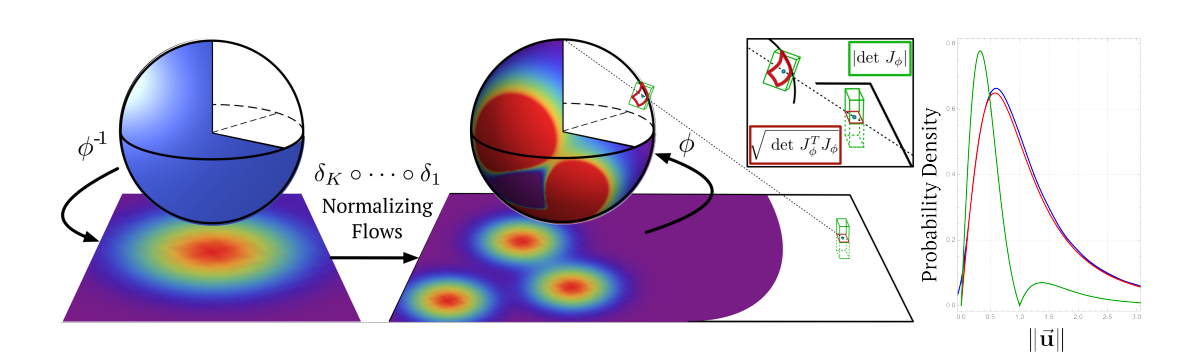
\includegraphics[width=\textwidth]{fig1.png}
    \caption{Слева: Конструкция сложной плотности на $S^n$ путем проецирования многообразия на $R^n$, преобразования плотности и обратного проецирования на $S^n$. Справа: Иллюстрация преобразованных ($S^2 \rightarrow R^2$) плотностей, соответствующих равномерной плотности на сфере. Синий: эмпирическая плотность (получена методом Монте-Карло); Красный: аналитическая плотность из уравнения (4); Зеленый: плотность, вычисленная без учета внутренней размерности $S^n$.}
    \label{fig:figure1}
\end{figure}

Эти специальные многообразия \( M \subset R^m \) гомеоморфны евклидовому пространству \( R^n \), где \( n \) соответствует размерности касательного пространства \( M \) в каждой точке. Гомеоморфизм — это непрерывная функция между топологическими пространствами с непрерывным обратным (биективная и бинепрерывная). Он отображает точки одного пространства в другое уникальным и непрерывным образом. Примером многообразия является единичная 2-сфера, поверхность единичного шара, которая вложена в \( R^3 \) и гомеоморфна \( R^2 \) (см. Рис. \ref{fig:figure1}).

В нормализующих потоках основной результат дифференциальной геометрии, используемый для вычисления обновлений плотности, задается \( d\hat{x} = |\det J_\phi| du \) и представляет собой связь между дифференциалами (бесконечно малыми объемами) между двумя равномерными евклидовыми пространствами с использованием якобиана функции \( \phi : R^n \rightarrow R^n \), которая преобразует одно пространство в другое. Этот результат применим только к преобразованиям, сохраняющим размерность. Однако преобразования, отображающие вложенное многообразие в его внутреннее евклидово пространство, не сохраняют размерность точек, и вышеуказанный результат становится неприменимым.

Якобиан таких преобразований \( \phi : R^n \rightarrow R^m \) с \( m > n \) является прямоугольным, и бесконечно малый куб на \( R^n \) отображается в бесконечно малый вырожденный параллелепипед на многообразии. Связь между этими объемами задается \( d\hat{x} = \sqrt{\det G_\phi} du \), где \( G_\phi = J_\phi^T J_\phi \) — метрика, индуцированная вложением \( \phi \) на касательное пространство \( T_xM \). Правильная формула для вычисления плотности над \( M \) теперь становится:

\begin{equation}
    \int_{M \subset R^m} f(\tilde{x}) d\hat{x} = \int_{R^n} (f \circ \phi)(\tilde{u}) \sqrt{\det G} du = \int_{R^n} (f \circ \phi)(\tilde{u}) \sqrt{\det J_\phi^T J_\phi} du
    \label{eq:density_update}
\end{equation}

Индуцированная риманова метрика \( G_\phi \) позволяет четко определять понятия кривизны, объема, градиентов функций и дивергенции векторных полей. Обновление плотности при переходе от многообразия к евклидовому пространству, \( \tilde{x} \in S^n \rightarrow \tilde{u} \in R^n \), задается:

\begin{equation}
    p(\tilde{u}) = (f \circ \phi)(\tilde{u}) \sqrt{\det J_\phi^T J_\phi(\tilde{u})} = f(\tilde{x}) \sqrt{\det J_\phi^T J_\phi(\phi^{-1}(\tilde{x}))}
    \label{eq:density_update_manifold}
\end{equation}

В качестве применения этого метода на \( n \)-сфере \( S^n \) мы вводим обратное стереографическое преобразование и определяем его как: \( \phi(u) : R^n \rightarrow S^n \subset R^{n+1} \),

\begin{equation}
    \tilde{x} = \phi(\tilde{u}) = \left( \frac{2u}{u^T u + 1}, \frac{1 - 2}{u^T u + 1} \right)
    \label{eq:inverse_stereographic}
\end{equation}

которое отображает \( R^n \) на \( S^n \) биективным и бинепрерывным образом. Определитель метрики \( G_\phi \), связанной с этим преобразованием, задается:

\begin{equation}
    \det G_\phi(x) = \det J_\phi(x)^T J_\phi(x) = \left( \frac{2}{x^T x + 1} \right)^{2n}
    \label{eq:det_metric}
\end{equation}

Используя эти формулы, на левой стороне Рис. \ref{fig:figure1}, мы отображаем равномерную плотность на \( S^2 \) на \( R^2 \), обогащаем эту плотность, например, с помощью нормализующих потоков, и затем отображаем ее обратно на \( S^2 \), чтобы получить многомодальную (или произвольно сложную) плотность на исходной сфере. На правой стороне Рис. \ref{fig:figure1} мы показываем, что обновление плотности на основе римановой метрики, т.е. \( \sqrt{\det J_\phi^T J_\phi} \) (красный), является правильным и тесно следует оценке ядерной плотности на основе 500k выборок (синий). Мы также показываем, что использование общей формулы преобразования объема для сохранения размерности, т.е. \( |\det J_\phi| \) (зеленый), приводит к ошибочной плотности и не похоже на эмпирические распределения выборок после преобразования.

\section{Вариационный автокодировщик}
Для данного набора данных \(\mathbf{x} = (x_1, x_2, \ldots, x_n)\) вариационный автокодировщик (VAE) стремится научиться непрерывной латентной переменной, которая максимизирует логарифм правдоподобия \(\log p(\mathbf{x}) = \log \int p_{\theta}(\mathbf{x} \mid \mathbf{z}) p(\mathbf{z}) d\mathbf{z}\). Поскольку эта маргинальная функция часто невычислима, вариационное распределение \(q_{\phi}(\mathbf{z} \mid \mathbf{x})\) используется для аппроксимации истинного постериорного распределения \(p_{\theta}(\mathbf{z} \mid \mathbf{x})\). VAE пытается максимизировать следующую нижнюю границу правдоподобия:

\[
\begin{aligned}
\mathcal{L}(\theta ; \phi ; \mathbf{x}) = & \mathbb{E}_{q(\mathbf{x})}\left[\mathbb{E}_{q_{\phi}(\mathbf{z} \mid \mathbf{x})}[\log p_{\theta}(\mathbf{x} \mid \mathbf{z})]\right. \\
& \left.-KL(q_{\phi}(\mathbf{z} \mid \mathbf{x}) \| p(\mathbf{z}))\right]
\end{aligned}
\]

где \(q(\mathbf{x})\) — эмпирическое распределение входных данных, а приор \(p(\mathbf{z})\) обычно предполагается стандартным гауссовым распределением для простоты. Первый член в объективе — это ошибка восстановления, а второй — KL-дивергенция.

\subsection{Проблема исчезновения KL-дивергенции}
Проблема исчезновения KL-дивергенции возникает потому, что генеративная модель часто является LSTM, которая обладает высокой выразительной способностью, что приводит к тому, что член восстановления в объективе доминирует над KL-дивергенцией. В этом случае модель способна генерировать тексты без эффективного использования латентных кодов, так как латентная переменная \(\mathbf{z}\) становится независимой от входных данных при схлопывании KL-дивергенции до нуля.

Существует два основных подхода для решения этой проблемы. Один из них заключается в исследовании различных вариантов декодерной модели для контроля выразительной способности LSTM. Другой подход заключается в изменении формы латентного распределения и модификации целевой функции обучения.

\section{Основные понятия}

В этом разделе мы рассмотрим основные концепции римановой геометрии, нормализующих потоков и вассерштейновского автокодировщика. Затем мы введем наш новый риманов нормализующий поток.

\subsection{Обзор римановой геометрии}
Рассмотрим входное пространство \(\mathcal{X} \subset \mathbb{R}^D\). \(d\)-мерное многообразие (\(d < D\)) — это гладкая поверхность точек, вложенная в \(\mathcal{X}\). Для данного многообразия \(\mathcal{M}\) риманово многообразие — это метрическое пространство \((\mathcal{M}, G)\), где \(G\) — риманов метрический тензор, который задает скалярное произведение в каждой точке многообразия. Более формально, риманов метрик \(G: \mathcal{Z} \rightarrow \mathbb{R}^{d \times d}\) определяется как гладкая функция, такая что для любых двух векторов \(u, v\) в касательном пространстве \(T_z M\) каждой точки \(z \in \mathcal{M}\) он задает следующее скалярное произведение для \(u\) и \(v\):

\[
\langle u, v \rangle_G = u^T G(z) v
\]

Риманов метрик помогает характеризовать многие внутренние свойства многообразия. Рассмотрим произвольную гладкую кривую \(\gamma(t): [a, b] \rightarrow \mathcal{M}\) на данном многообразии \(\mathcal{M}\) с римановым метрическим тензором \(G\). Длина этой кривой определяется как:

\[
\begin{aligned}
\mathcal{L}(\gamma) & = \int_{a}^{b} \left\| \gamma'(t) \right\| dt \\
& = \int_{a}^{b} \sqrt{\langle \gamma_t', \gamma_t' \rangle_G} dt \\
& = \int_{a}^{b} \sqrt{\gamma_t'^T G(\gamma_t) \gamma_t'} dt
\end{aligned}
\]

где \(\gamma_t'\) — скорость кривой и лежит в касательном пространстве \(T_{\gamma_t} M\) в точке \(\gamma(t)\). Когда метрический тензор \(G\) равен 1 повсюду на кривой, он становится метрическим тензором в евклидовом пространстве, где длина кривой определяется как интеграл от функции скорости: \(\mathcal{L}(\gamma) = \int_{a}^{b} \sqrt{\gamma_t'} \gamma_t' dt = \int_{a}^{b} \gamma_t' dt\).

Геодезическая линия между любыми двумя точками определяется как кривая, минимизирующая длину кривой \(\gamma\). Например, если \(\gamma_t\) — геодезическая кривая, соединяющая \(\gamma(a)\) и \(\gamma(b)\), то:

\[
\gamma_t = \underset{\gamma}{\operatorname{argmin}} \mathcal{L}(\gamma)
\]

Практически геодезическая линия часто находится путем оптимизации следующей функции энергии:

\[
\begin{aligned}
E(\gamma) & = \frac{1}{2} \int_{a}^{b} \gamma_t'^T G(\gamma_t) \gamma_t' dt \\
\gamma_t & = \underset{\gamma}{\operatorname{argmin}} E(\gamma)
\end{aligned}
\]

Отметим, что евклидов метрик является частным случаем риманова метрика. Более общий метрический тензор \(G\) дает представление о том, насколько риманова геометрия отклоняется от евклидовой геометрии.

\subsection{Обзор: Нормализующие потоки}
Мощная инференсная модель VAE может аппроксимировать истинное постериорное распределение через вариационное выведение. Выбор этой аппроксимированной постериорной функции является одной из основных проблем. Для вычислительной эффективности диагональное гауссово распределение часто выбирается в качестве формы постериорного распределения. Поскольку ковариационная матрица всегда предполагается диагональной, постериорное распределение не может захватывать зависимости между отдельными измерениями латентных кодов. Это ставит сложную задачу в вариационном выведении. Поскольку маловероятно, что истинное постериорное распределение имеет диагональную форму, аппроксимированное диагональное распределение недостаточно гибкое, чтобы соответствовать истинному постериорному распределению даже в асимптотическом времени.

Нормализующий поток, разработанный Rezende и Mohamed (2015), вводится для преобразования простого постериорного распределения в более гибкое распределение. Формально, серия нормализующих потоков — это набор обратимых гладких преобразований \(f_t: \mathbb{R}^d \rightarrow \mathbb{R}^d\) для \(t = 1, \ldots, T\), таких что для данной случайной величины \(z_0\) с распределением \(q(z_0)\) результирующая случайная величина \(z^T = (f_T \circ f_{T-1} \circ \ldots \circ f_1)(z_0)\) имеет следующую функцию плотности:

\[
q(z_T) = q(z_0) \prod_{t=1}^{T} \left| \det \frac{\partial f_t^{-1}}{\partial z_{t-1}} \right|
\]

Поскольку каждое преобразование \(f_i\) для \(i = 1, \ldots, T\) обратимо, его якобиан детерминант существует и может быть вычислен. Оптимизируя модифицированную нижнюю границу правдоподобия:

\[
\begin{aligned}
\ln p(x) \geq \mathbb{E}_{q(z_0 \mid x)} & \left[ \ln p(x \mid z_T) + \sum_{t=1}^{T} \ln \left| \det \frac{\partial f_t}{\partial z_{t-1}} \right| \right] \\
& - KL(q(z_0 \mid x) \| p(z_T))
\end{aligned}
\]

результирующие латентные коды \(z_T\) будут иметь более гибкое распределение.

На основе того, как вычисляется якобиан детерминант, существует два основных семейства нормализующих потоков (Tomczak и Welling, 2016; Berg и др., 2018): общие нормализующие потоки и потоки с сохранением объема. Оба они ищут гибкое преобразование с легко вычисляемым якобианом детерминантом, но поток с сохранением объема направлен на нахождение специфического потока, якобиан детерминант которого равен 1, что упрощает задачу оптимизации в уравнении (6). Поскольку мы хотим получить нормализующий поток, который не только дает гибкое постериорное распределение, но и способен раскрыть истинные геометрические свойства латентного пространства, мы рассматриваем только общие нормализующие потоки, якобиан детерминант которых не является константой, так как нам нужно моделировать риманов метрик, введенный ранее.

\section{Вассерштейновский автокодировщик}
Вассерштейново расстояние было введено в генеративные модели и показало свою успешность в многих задачах генерации изображений (Tolstikhin и др., 2018; Arjovsky и др., 2017; Bousquet и др., 2017). Вместо максимизации нижней границы правдоподобия, как это делает VAE, вассерштейновский автокодировщик (WAE) (Tolstikhin и др., 2018) оптимизирует затраты на оптимальную транспортировку (Villani, 2008) между истинным распределением данных \(P_X(x)\) и генеративным распределением \(P_G(x)\). Это приводит к вассерштейновскому объективу:

\[
\begin{aligned}
D(P_X, P_G) = \inf_{Q(Z \mid X) \in \mathcal{Q}} \mathbb{E}_{P_X} \mathbb{E}_{Q(Z \mid X)}[c(X, G(Z))] + \lambda D_Z(Q_Z, P_Z)
\end{aligned}
\]

где \(c(\cdot)\) — затраты на оптимальную транспортировку, \(G: \mathcal{Z} \rightarrow \mathcal{X}\) — любая генеративная функция, а коэффициент \(\lambda\) контролирует силу регуляризационного члена \(D_Z\). При заданном положительно определенном воспроизводящем ядре \(k: \mathcal{Z} \times \mathcal{Z} \rightarrow \mathbb{R}\) регуляризационный член \(D_Z\) может быть аппроксимирован максимальным средним расхождением (MMD) (Gretton и др., 2012) между приором \(P_Z\) и агрегированным постериорным распределением \(Q_Z(z) = \int q(z \mid x) p(x) dx\):

\[
MMD_k(P_Z, Q_Z) = \left\| \int_{\mathcal{Z}} k(z, \cdot) dP_Z - \int_{\mathcal{Z}} k(z, \cdot) dQ_Z \right\|
\]

\subsection{Максимальное среднее расхождение (MMD)}

Максимальное среднее расхождение (MMD) — это мера расстояния между двумя вероятностными распределениями на основе их вложений в воспроизводящее ядерное пространство Гильберта (RKHS). Для двух распределений \(P\) и \(Q\) и положительно определенного ядра \(k\) MMD определяется как:

\[
MMD_k(P, Q) = \left\| \mathbb{E}_P[k(z, \cdot)] - \mathbb{E}_Q[k(z, \cdot)] \right\|_{\mathcal{H}}
\]

где \(\mathcal{H}\) — RKHS, связанное с ядром \(k\). MMD можно оценить эмпирически с использованием выборок из распределений \(P\) и \(Q\):

\[
MMD_k(P, Q) \approx \left[ \frac{1}{m^2} \sum_{i,j=1}^m k(z_i, z_j) + \frac{1}{n^2} \sum_{i,j=1}^n k(z_i', z_j') - \frac{2}{mn} \sum_{i=1}^m \sum_{j=1}^n k(z_i, z_j') \right]^{\frac{1}{2}}
\]

где \(z_i \sim P\) и \(z_j' \sim Q\).

Выбор ядра \(k\) критически важен для производительности MMD. Распространенные выборы включают гауссово ядро \(k(z, z') = \exp(-\frac{\|z - z'\|^2}{2\sigma^2})\) и лапласов ядро \(k(z, z') = \exp(-\frac{\|z - z'\|}{\sigma})\). Параметр ширины полосы \(\sigma\) контролирует чувствительность ядра к расстоянию между выборками.

\section{Наш подход}

В этом разделе мы предлагаем наш риманов нормализующий поток (RNF). RNF — это новый тип потока, который использует риманов метрический тензор, введенный ранее. Этот метрик заставляет стохастический кодировщик учить более богатый класс аппроксимированных постериорных распределений, чтобы следовать истинной геометрии латентного пространства, что помогает избежать локального оптимума, в котором постериорное распределение схлопывается в стандартный приор. Затем мы объединяем это с WAE и объясним, почему и как WAE следует использовать для обучения с RNF.

\subsection{Риманов нормализующий поток}
В контексте VAE обучение латентного пространства, гомеоморфного входному пространству, часто является очень сложной задачей. Рассмотрим многообразие \(\mathcal{M} \subset \mathbb{R}^D\). Генераторная модель \(x = f(z): \mathcal{Z} \rightarrow \mathbb{R}^D\) служит низкоразмерной параметризацией многообразия \(\mathcal{M}\) относительно \(z \in \mathcal{Z}\). В большинстве случаев латентное пространство \(\mathcal{Z}\) маловероятно является гомеоморфным \(\mathcal{M}\), что означает, что не существует обратимого отображения между \(\mathcal{M}\) и \(\mathcal{Z}\). И поскольку инференсная модель \(h: \mathcal{M} \rightarrow \mathcal{Z}\) нелинейна, выученное латентное пространство часто дает искаженное представление входного пространства. Рассмотрим случай на рисунке 2, где левый график — это входное многообразие, а правый график — это соответствующее латентное пространство с кривизной, отраженной яркостью. Возьмем две произвольные точки на многообразии и найдем геодезическую линию, соединяющую эти две точки. Если мы рассматриваем искаженное латентное пространство как евклидово, то геодезическая линия в латентном пространстве не отражает истинное кратчайшее расстояние между этими двумя точками на многообразии, так как прямая линия в латентном пространстве пересекала бы все многообразие, тогда как истинная геодезическая линия должна была бы обходить эту дыру. Это искажение вызвано непостоянной кривизной латентного пространства. Следовательно, латентное пространство следует рассматривать как кривое пространство с кривизной, отраженной римановым метриком, определенным локально вокруг каждой точки. Как указано яркостью, мы видим, что центральная область латентного пространства сильно искривлена и, следовательно, имеет более высокую энергию. Геодезическая линия, соединяющая два латентных кода, минимизирует функцию энергии \(E(\gamma) = \frac{1}{2} \int \gamma_t'^T G(\gamma_t) \gamma_t' dt\), что указывает на то, что она должна избегать тех областей с высокой кривизной \(G\).

Теперь вопрос заключается в том, как навязать эту внутреннюю метрику и кривизну латентному пространству. В этой статье мы предлагаем новую форму нормализующего потока для инкорпорации с этой геометрической характеристикой. Сначала рассмотрим нормализующий поток \(f: \mathcal{Z} \rightarrow \mathcal{Z}'\). Мы можем вычислить длину кривой в преобразованном латентном пространстве \(\mathcal{Z}'\):

\[
\begin{aligned}
\mathcal{L}(f(\gamma_t)) & = \int_{a}^{b} \left\| \mathbf{J}_{\gamma_t} \gamma_t' \right\| dt \\
& = \int_{a}^{b} \sqrt{\gamma_t' \mathbf{J}_{\gamma_t}^T \mathbf{J}_{\gamma_t} \gamma_t'} dt \\
& = \int_{a}^{b} \sqrt{\gamma_t' G(\gamma_t) \gamma_t'} dt
\end{aligned}
\]

где

\[
\begin{aligned}
\gamma_t & : [a, b] \rightarrow \mathcal{Z}', \quad a, b \in \mathcal{Z} \\
\mathbf{J}_{\gamma_t} & = \left. \frac{\partial f}{\partial \mathbf{z}} \right|_{\mathbf{z} = \gamma_t} \\
G(\gamma_t) & = \mathbf{J}_{\gamma_t}^T \mathbf{J}_{\gamma_t} \\
& = \left. \left( \frac{\partial f}{\partial \mathbf{z}} \right)^T \left( \frac{\partial f}{\partial \mathbf{z}} \right) \right|_{\mathbf{z} = \gamma_t}
\end{aligned}
\]

\(\mathbf{J}_{\gamma_t}\) — это матрица Якоби, определенная в \(\gamma_t\). В нашем случае риманов метрический тензор \(G\) является скалярным произведением Якоби \(\mathbf{J}_{\gamma_t}\) и, следовательно, симметричен положительно определен. Он отражает кривизну входного пространства в низкоразмерной параметризации \(\mathcal{Z}'\). В области с высокой кривизной метрический тензор \(G = \mathbf{J}^T \mathbf{J}\) больше, чем в других областях, что указывает на то, что латентное представление входного многообразия имеет меньшую кривизну или область низкой энергии, так как любая геодезическая линия, соединяющая каждую пару точек на многообразии, предпочитает путь с меньшей энергией. Это означает, что те области вне области данных многообразия должны иметь высокую кривизну в латентном пространстве.

В этой статье мы вводим риманов нормализующий поток (RNF) для моделирования кривизны. Для простоты мы строим нашу модель на основе планарного потока (Rezende и Mohamed, 2015). Планарный поток — это обратимое преобразование, которое сжимает и растягивает область оригинального латентного пространства относительно плоскости. Математически планарный поток \(f: \mathcal{Z} \rightarrow \mathcal{Z}'\) имеет вид:

\[
f(\mathbf{z}) = \mathbf{z} + \mathbf{u} h(\mathbf{w}^T \mathbf{z} + b)
\]

где \(h: \mathbb{R}^d \rightarrow \mathbb{R}^d\) — любая гладкая нелинейная функция и часто выбирается как \(\tanh(\cdot)\). Условие обратимости выполняется, если \(\mathbf{u}^T \mathbf{w} \geq -1\). Его якобиан детерминант относительно латентных кодов \(\mathbf{z}\) легко вычислить:

\[
\begin{aligned}
\left| \det \frac{\partial f}{\partial \mathbf{z}} \right| & = \left| 1 + \mathbf{u}^T \phi(\mathbf{z}) \mathbf{w} \right| \\
\phi(\mathbf{z}) & = h'(\mathbf{w}^T z + b)
\end{aligned}
\]

С детерминантом Якоби от планарного потока легко вычислить детерминант метрического тензора \(G\). Чтобы увидеть это, отметим, что поскольку \(\frac{\partial f}{\partial \mathbf{z}}: \mathbb{R}^d \rightarrow \mathbb{R}^d\) — квадратная матрица с полным столбцовым рангом благодаря обратимости \(f\), мы имеем:

\[
\left| \det G \right| = \left| \frac{\partial f^T}{\partial \mathbf{z}} \right| \left| \frac{\partial f}{\partial \mathbf{z}} \right| = \left| \frac{\partial f}{\partial \mathbf{z}} \right|^2
\]

Для обеспечения хорошо определенной геометрии в преобразованном латентном пространстве нам нужен якобиан детерминант \(\left| \frac{\partial f}{\partial \mathbf{z}} \right|\), который велик в области с высокой кривизной \(\left| \det G \right|\). Таким образом, мы предлагаем моделировать метрический тензор с помощью обратной мультиквадратичной функции ядра \(\mathcal{K}\), использованной Tolstikhin и др. (2018), и гауссовым ядром, то есть:

\[
\begin{aligned}
\mathcal{K}_m(\mathbf{z}, \mathbf{c}_k) & = C / (C + \left\| \mathbf{z} - \mathbf{c}_k \right\|_2^2) \\
\mathbf{k} & = \operatorname{argmin} \left\| \mathbf{z} - \mathbf{c}_k \right\|_2^2 \\
\mathcal{K}_g(\mathbf{z}, \mathbf{c}_k) & = \exp(-\beta_k \left\| \mathbf{z} - \mathbf{z}_k \right\|_2^2)
\end{aligned}
\]

где \(\mathbf{c}_k, k = 1, 2, 3, \ldots, K\) — кластеры латентных кодов, а \(\beta_k\) — ширина полосы. Мы наблюдаем, что обратная мультиквадратичная функция ядра \(\mathcal{K}_m\) обычно работает лучше. Мы используем вышеуказанные ядра в качестве ограничений на якобиан детерминант, так что:

\[
\left| \det \frac{\partial f'}{\partial \mathbf{z}} \right| = \left| 1 + \mathbf{u}^T(\mathbf{z}) \phi(\mathbf{z}) \mathbf{w} \right| \cdot \mathcal{K}(\mathbf{z}, \mathbf{c}_k)
\]

Как мы объяснили ранее в этом разделе, латентное представление области вне входного многообразия должно иметь высокую кривизну в латентном пространстве. Во время обучения мы стремимся максимизировать этот регуляризованный якобиан \(\left| \det \frac{\partial f'}{\partial \mathbf{z}} \right|\), а не оригинальный. Это обеспечивает, что те латентные коды внутри латентных кластеров и, следовательно, вероятно, находящиеся на или около входного многообразия во входном пространстве, имеют гораздо меньшую кривизну \(\left| \det G \right| = \left| \frac{\partial f}{\partial \mathbf{z}} \right|^2\), чем те вне латентных кластеров, так как те вне многообразия будут стремиться к большему якобиану, чтобы компенсировать регуляризационный член \(\mathcal{K}\). Латентное пространство \(\mathcal{Z}'\), преобразованное нормализующим потоком \(f\), таким образом, искривлено относительно входного многообразия. Этот тип нормализующего потока, таким образом, учит латентное пространство, которое уважает геометрические характеристики входного пространства. Проблема исчезновения KL маловероятна с искривленным латентным пространством. Это потому, что большинство высокоразмерных данных в реальной жизни образуют искривленное многообразие, которое маловероятно выбирается из многомерного стандартного гауссова распределения. Тогда, если латентное пространство отражает кривизну искривленного многообразия, область опор латентных кодов, безусловно, не следует стандартному гауссову распределению. Это помогает отталкивать постериорное распределение \(q(\mathbf{z} \mid \mathbf{x})\) от стандартного гауссова распределения и никогда не схлопываться в неинформативный приор.

\subsection{RNF Вассерштейновский автокодировщик}
Здесь мы рассматриваем использование вассерштейновского объектива для моделирования маргинального латентного распределения искривленного латентного пространства, выученного RNF. Вассерштейновский объектив с MMD привлекателен в нашем случае по двум основным причинам.

Во-первых, вместо минимизации KL-дивергенции \(KL(q(\mathbf{z} \mid \mathbf{x}) \| p(\mathbf{z}))\), он минимизирует расстояние между \(q(\mathbf{z}) = \int q(\mathbf{z} \mid \mathbf{x}) p(\mathbf{x}) dx\) и \(p(\mathbf{z})\), что поощряет маргинальное распределение латентного пространства быть как можно ближе к приору, не затрагивая при этом индивидуальное постериорное распределение \(q(\mathbf{z} \mid \mathbf{x})\), условленное каждым входом. Это делает KL-дивергенцию между постериорным и приорным распределениями и, эквивалентно, взаимную информацию между латентными кодами и входными предложениями \(I(\mathbf{z}, \mathbf{x}) = KL(q(\mathbf{z}, \mathbf{x}) \| q(\mathbf{z}) p(\mathbf{x})) = \mathbb{E}_{p(\mathbf{x})}[KL(q(\mathbf{z} \mid \mathbf{x}) \| p(\mathbf{z}))] - KL(q(\mathbf{z}) \| p(\mathbf{z}))\) невозможной для исчезновения, так как объектив не требует, чтобы она была маленькой. Поскольку выученные латентные коды и входные предложения имеют ненулевую взаимную информацию, генеративная модель не будет игнорировать латентные коды при генерации текстов.

Во-вторых, MMD-регуляризация в WAE делает возможным оптимизацию нормализующего потока без явного вычисления якобиан детерминанта. Использование MMD необходимо, так как получить замкнутую форму KL-дивергенции больше невозможно после применения RNF к постериорному распределению. И поскольку генеративная функция \(G\) в члене восстановления вассерштейновского объектива может быть любой функцией или композицией функций (Tolstikhin и др., 2018), мы можем легко составить функцию RNF в \(G\), так что восстановленные тексты \(\bar{X} = G(f(Z)) = G(Z'), Z' \in \mathcal{Z}'\), \(Z' = F(Z)\).

Теперь, при заданной серии RNF \(F = f_K \circ \ldots \circ f_1\) и \(\mathcal{Z}_K\) — искривленное латентное пространство после применения \(K\) потоков к оригинальному латентному пространству \(\mathcal{Z}\), мы оптимизируем следующий RNF-вассерштейновский объектив:

\[
\begin{aligned}
D(P_X, P_G) = & \inf_{Q(Z \mid X) \in \mathcal{Q}} \mathbb{E}_{P_X} \mathbb{E}_{Q(Z \mid X)}[c(X, G(Z'))] \\
& + \lambda MMD(Q_{Z'}, P_{Z'}) \\
& + \alpha (KL(q(\mathbf{z} \mid \mathbf{x}) \| p(\mathbf{z})) - \sum \log \left| \det \frac{\partial f'}{\partial \mathbf{z}} \right|)
\end{aligned}
\]

где \(Z \sim \mathcal{Z}\), \(Z' \sim \mathcal{Z}'\) и \(Z' = F(Z)\). Мы аппроксимируем член MMD с гауссовым ядром \(k(\mathbf{z}, \mathbf{z}') = e^{-\|\mathbf{z} - \mathbf{z}'\|^2}\), то есть \(MMD(p, q) = \mathbb{E}_{p(\mathbf{z}), p(\mathbf{z}')}[k(\mathbf{z}, \mathbf{z}')] + \mathbb{E}_{q(\mathbf{z}), q(\mathbf{z}')}[k(\mathbf{z}, \mathbf{z}')] - 2 \mathbb{E}_{p(\mathbf{z}), q(\mathbf{z}')}[k(\mathbf{z}, \mathbf{z}')]\).

Здесь мы выбираем минимизировать расстояние MMD между приором \(P_Z\) и маргиналом неискривленного латентного пространства. Это делает процедуру выборки для задач генерации гораздо проще, так как легко выбрать латентный код из неинформативного приора. Мы можем получить выборку \(\mathbf{z}'\) из \(\mathcal{Z}'\) косвенно, выбрав \(\mathbf{z} \sim P_Z(\mathbf{z})\) и \(\mathbf{z}' \sim F(\mathbf{z})\). С другой стороны, было бы гораздо сложнее выбрать напрямую из искривленного латентного пространства \(\mathcal{Z}'\), так как единственное приорное знание, которое у нас есть о \(\mathcal{Z}'\), — это кривизна, отраженная RNF неявно, и, следовательно, мы не знаем опору \(Q(Z')\).

\section{Заключение}
В этой статье мы ввели римановы нормализующие потоки для обучения вассерштейновского автокодировщика для моделирования текста. Эта новая модель поощряет выученные латентные представления текстов уважать геометрические характеристики пространства входных предложений. Наши результаты показывают, что RNF WAE значительно улучшает результаты моделирования языка за счет моделирования римановой геометрической пространства через нормализующие потоки.


\end{document}
